% !TEX encoding = UTF-8 Unicode
% !TEX root = ../../relatorio.tex

%% Responsavel:

\subsection{Questão 3.16}

Suppose \texttt{comm\_sz} = 8 and the vector x = (0, 1, 2, ... , 15) has been distributed among the processes using a block distribution. Draw a diagram illustrating the steps in a butterfly implementation of allgather of x. \\


\begin{figure}[h!]
  \begin{center}
    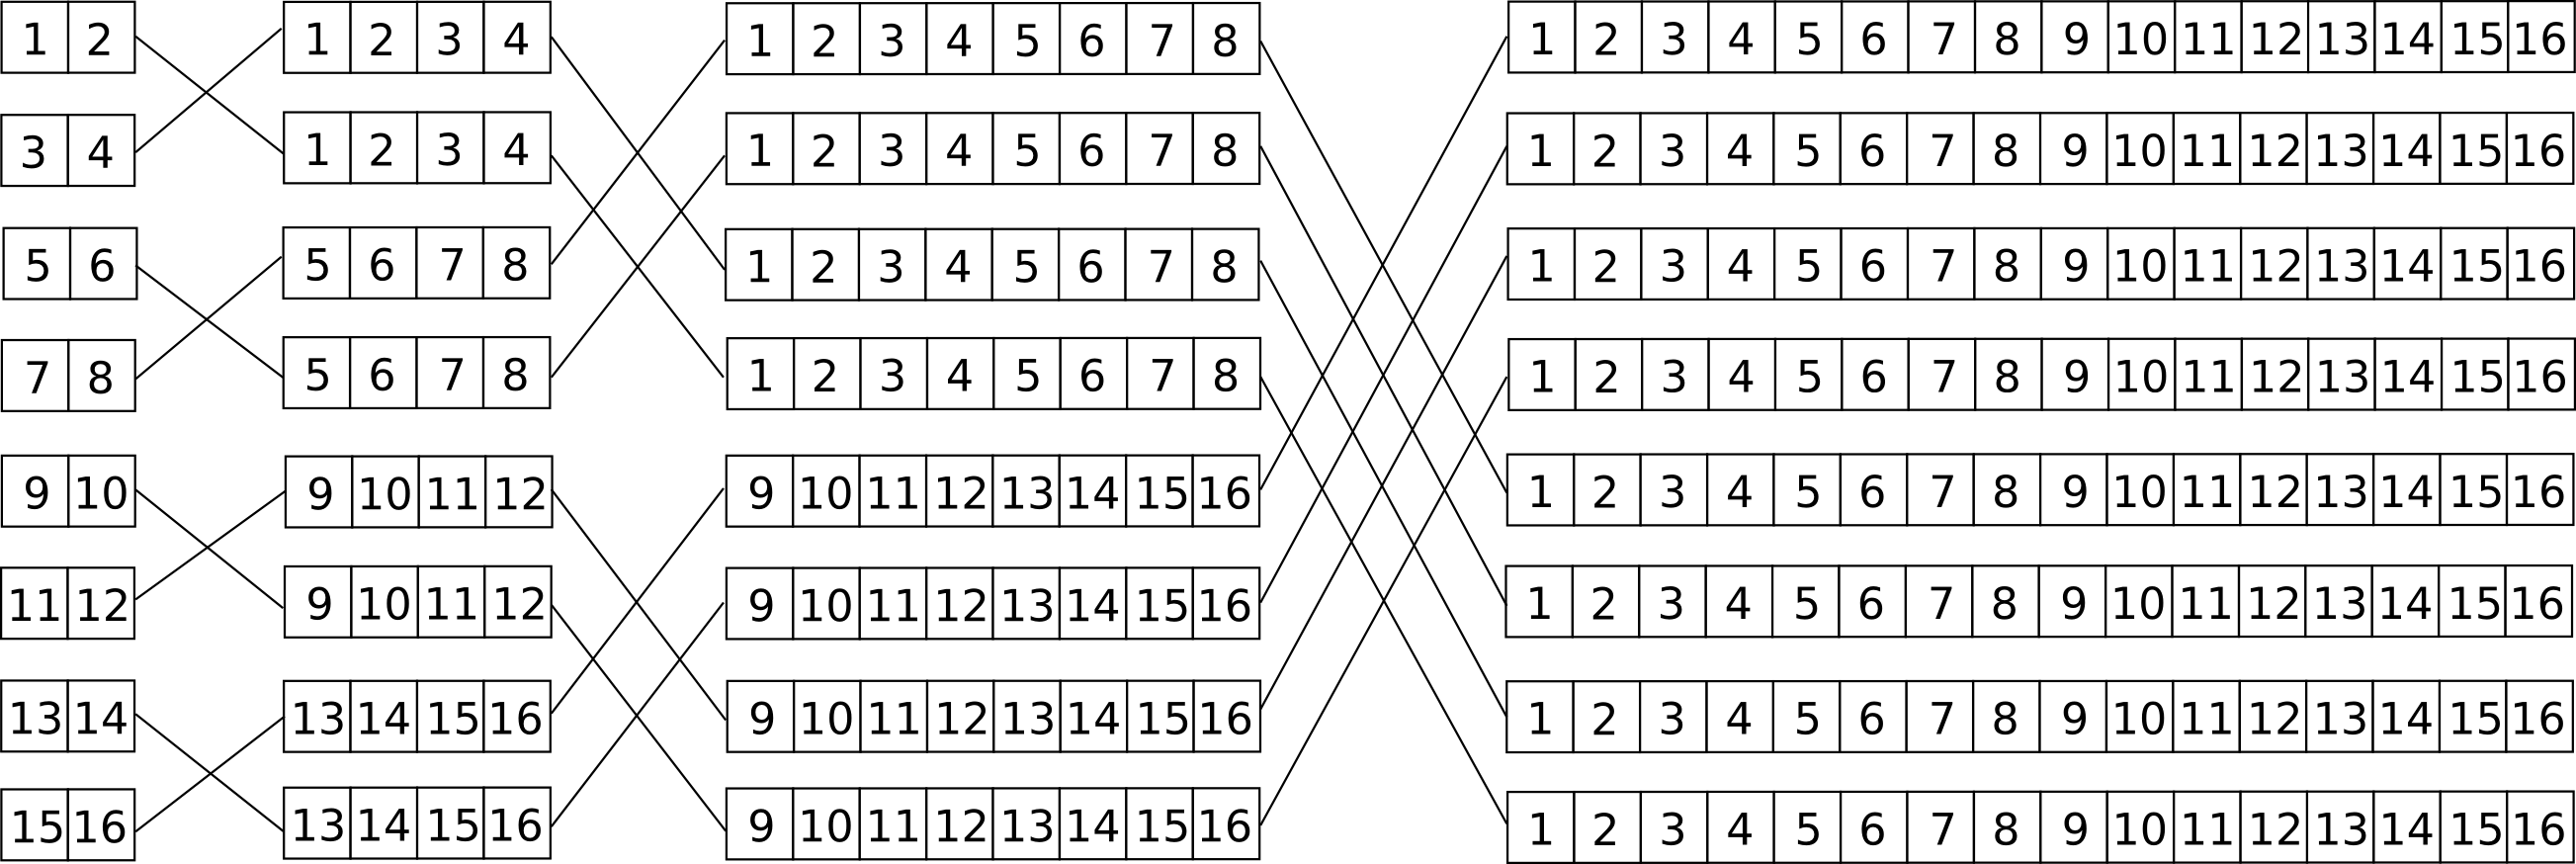
\includegraphics[width=450pt]{sections/q3.16/imgs/g1.png}
  \end{center}
  \caption{Allgather em comunicação butterfly}
  \label{fig:allgatherbutterfly}
\end{figure}


%%% Local Variables:
%%% mode: latex
%%% TeX-master: "../../relatorio"
%%% End:
